%%%%%%%%%%%%%%%%%%%%%%%%%%%%%%%%%%%%%%%%%%%%%%%%%%%%%%%%
% IE 643 Course Project poster, team InTra.
% Built on the course template (IE643_Poster_Template.tex, a0poster class by
% Gerlinde Kettl and Matthias Weiser, design by Timothy Kodikara, CC BY-NC-SA 3.0).
%%%%%%%%%%%%%%%%%%%%%%%%%%%%%%%%%%%%%%%%%%%%%%%%%%%%%%%%
\documentclass[a0,portrait]{a0poster}
\usepackage[top=5cm, bottom=0.3cm, left=3.45cm, right=4.55cm]{geometry}
\usepackage[compact]{titlesec}
\usepackage{multicol}
\columnsep=100pt
\columnseprule=15pt
\usepackage[svgnames]{xcolor}
\usepackage{palatino}
\usepackage{xkeyval}
\usepackage{graphicx}
\setlength{\abovecaptionskip}{5pt plus 5pt minus 3pt}
\graphicspath{{figures/}}
\usepackage{booktabs}
\usepackage[font=small,labelfont=bf]{caption}
\usepackage{amsfonts, amsmath, amsthm, amssymb}
\usepackage{csquotes}
\usepackage{wrapfig}
\usepackage{multirow}
\usepackage{makecell}
\def\columnseprulecolor{\color{NavyBlue}}%
\usepackage{framed}
\colorlet{frameborder}{NavyBlue}
\usepackage{tikz}
\usetikzlibrary{arrows.meta,positioning,shapes.geometric,fit,calc}
\usepackage{qrcode}
\usepackage{enumitem}
\setlist[itemize]{leftmargin=1.4em,itemsep=0.15em,topsep=0.3em}
\usepackage[hyphens]{url}
\def\UrlBreaks{\do\/\do-\do_\do.}
\renewcommand{\arraystretch}{1.15}
\newcommand{\good}[1]{\textbf{\color{DarkGreen}#1}}
% ---- links for the QR codes -------------------------------------------------------------
\newcommand{\repourl}{https://github.com/aksh10-at/InTra-IE643}
\newcommand{\demourl}{https://drive.google.com/file/d/1GM-y0Mdh6S_8vNPYg1NoYMK0SRUTaTso/view?usp=sharing}
%----------------------------------------------------------------------------------------
\begin{document}
\begin{minipage}[c]{\linewidth}
\vspace{0.1cm}
\noindent\makebox[\textwidth][c]{
\begin{minipage}[c]{0.14\linewidth}
\vspace{0pt}\raggedright
\hspace{1cm}

\includegraphics[scale=1.3,width=\linewidth]{figures/logo.png}
\end{minipage}
\hfill
\begin{minipage}[c]{0.75\textwidth}
\centering
\Huge \color{Green} \textbf{IE643 Course Project}\\[0.5cm]
\Huge \color{NavyBlue} \textbf{From Handwritten Lecture Notes to Structured PDFs}\\[0.35cm]
\LARGE \color{NavyBlue} \textbf{Team InTra}\\[0.4cm]
\Large \color{Black} \textbf{Ishaan Mane $^{1}$ (25M1522), Akshat Verma $^{2}$ (25M1527)}\\[0.3cm]
\normalsize \text{25m1522@iitb.ac.in$^{1}$, 25m1527@iitb.ac.in$^{2}$}\\
\large \color{Green} \textbf{}\\
\end{minipage}
\begin{minipage}[c]{0.145\textwidth}
\vspace{0pt}\raggedleft

\includegraphics[scale=1.3,width=\linewidth]{figures/IE643-Logo.pdf}
\hspace{1cm}
\end{minipage}}
\\[0.1cm]%
\color{NavyBlue}\setlength\FrameRule{25pt}
\begin{framed}
\vspace{0.1cm}
\raggedcolumns
\begin{multicols}{2}
%----------------------------------------------------------------------------------------
\color{Black}\small
\section*{Abstract}
We turn photos and scans of handwritten lecture notes into searchable PDFs with typeset equations
and the original drawings. A Qwen2.5-VL-7B vision-language model, fine-tuned with QLoRA on our own
410-page dataset, writes each page as Markdown with \LaTeX{} maths, Surya locates the drawings, and
deterministic code builds the PDF without adding content. Fine-tuning halves the transcription error
(NED 0.596 $\to$ 0.311). For the novelty phase we traced the wrong figures on dense notebook pages to
the step that pairs descriptions with drawings and fixed it: the right drawing now appears for 23 of
23 checked descriptions, up from 15. A live web demo runs the full pipeline.

%----------------------------------------------------------------------------------------
\section*{Introduction}
\begin{itemize}
	\item Handwritten notes kept as photos are hard to search or share, and retyping maths is slow.
	\item Classic OCR fails on handwriting, maths and layout. A vision-language model reads the
	whole page and can write structure (headings, lists, \LaTeX) directly.
	\item Two parts must agree: one model knows \emph{what} each drawing shows (it writes a
	description), another knows \emph{where} it is (a box). Pairing them is the hard step on dense
	notebook pages.
\end{itemize}
We outline our main \textbf{contributions}:
\begin{itemize}
	\item A 410-page dataset of handwritten notes from four sources, labelled as Markdown + \LaTeX.
	\item A fine-tuned recogniser (QLoRA, 0.57\% of parameters trained) and a deterministic PDF
	builder that never adds content (529 of 529 blocks kept on test).
	\item A stage-by-stage diagnosis of figure errors and a fix, \textbf{Method B}: ``Surya decides
	where, Qwen decides which'', checked blind, now running in our live web demo (Notes2PDF).
\end{itemize}

%----------------------------------------------------------------------------------------
\section*{Workflow}
Figure \ref{workflow} shows how the project progressed, from the dataset to the novelty work.
\begin{center}
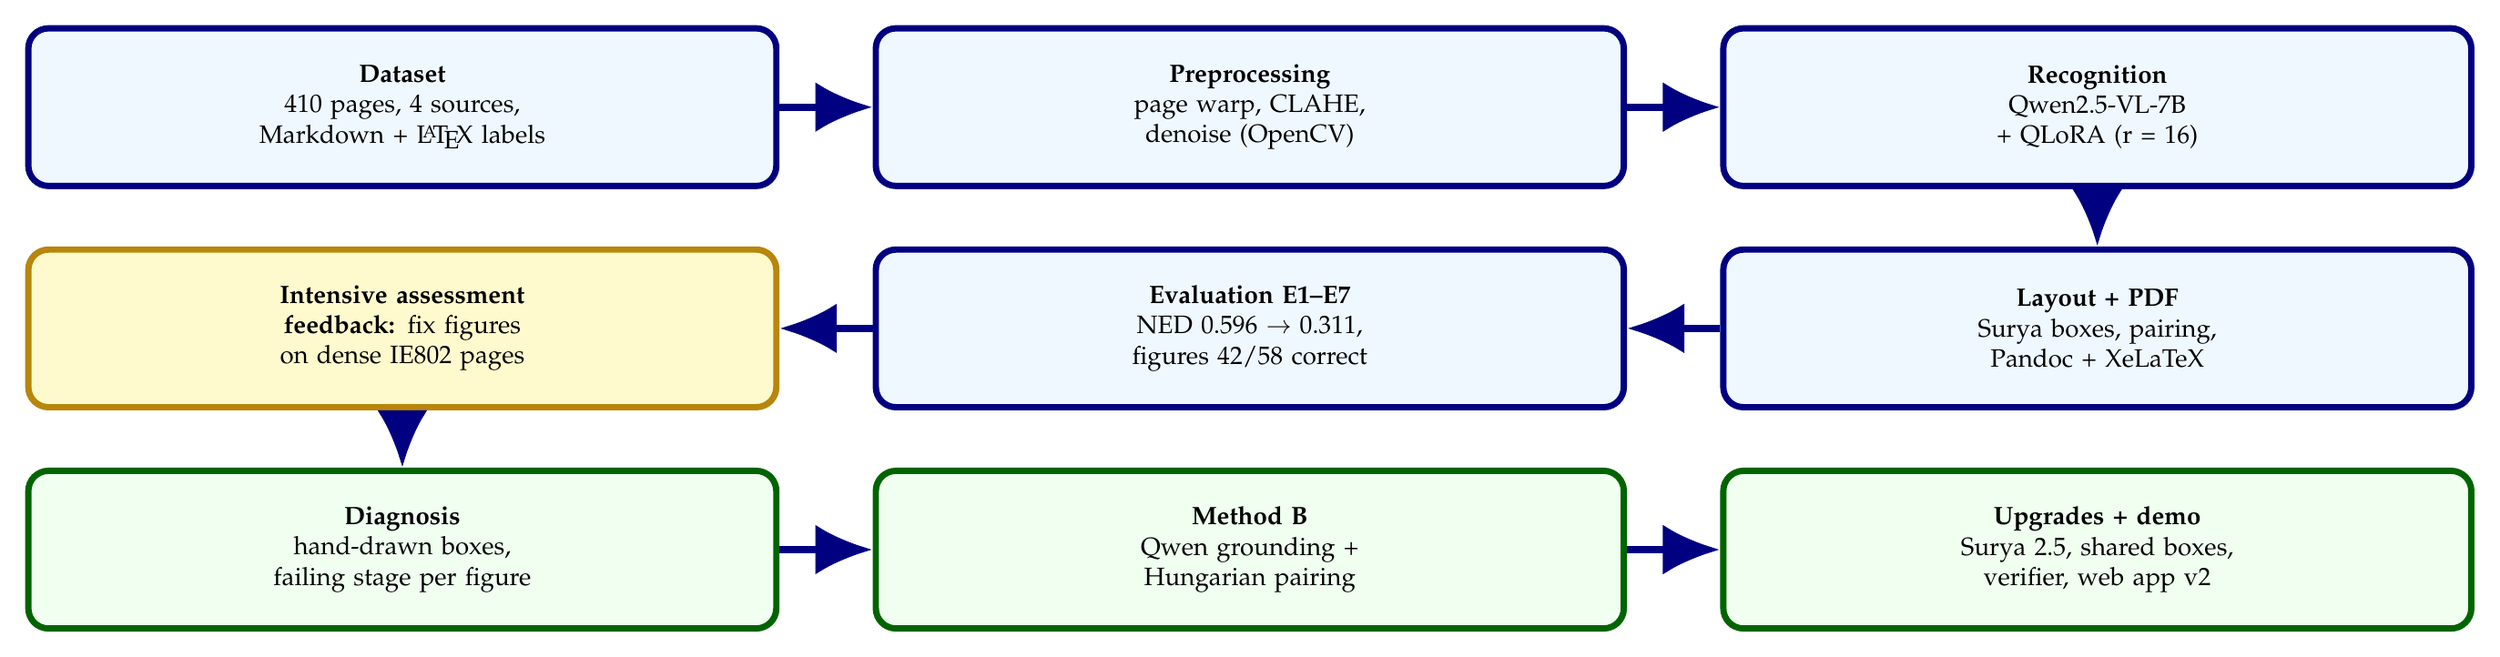
\begin{tikzpicture}[
  node distance=0.8cm and 1.3cm,
  box/.style={draw=NavyBlue, line width=2.5pt, rounded corners=8pt, fill=AliceBlue, align=center,
              minimum height=2.2cm, text width=10.2cm},
  nov/.style={box, fill=Honeydew, draw=DarkGreen},
  fb/.style={box, fill=LemonChiffon, draw=DarkGoldenrod},
  arr/.style={-{Latex[length=0.8cm,width=0.7cm]}, line width=3pt, NavyBlue}]
  \node[box] (d) {\textbf{Dataset}\\410 pages, 4 sources,\\Markdown + \LaTeX{} labels};
  \node[box, right=of d] (p) {\textbf{Preprocessing}\\page warp, CLAHE,\\denoise (OpenCV)};
  \node[box, right=of p] (r) {\textbf{Recognition}\\Qwen2.5-VL-7B\\+ QLoRA (r = 16)};
  \node[box, below=of r] (l) {\textbf{Layout + PDF}\\Surya boxes, pairing,\\Pandoc + XeLaTeX};
  \node[box, left=of l] (e) {\textbf{Evaluation E1--E7}\\NED 0.596 $\to$ 0.311,\\figures 42/58 correct};
  \node[fb, left=of e] (f) {\textbf{Intensive assessment}\\\textbf{feedback:} fix figures\\on dense IE802 pages};
  \node[nov, below=of f] (g) {\textbf{Diagnosis}\\hand-drawn boxes,\\failing stage per figure};
  \node[nov, right=of g] (m) {\textbf{Method B}\\Qwen grounding +\\Hungarian pairing};
  \node[nov, right=of m] (u) {\textbf{Upgrades + demo}\\Surya 2.5, shared boxes,\\verifier, web app v2};
  \draw[arr] (d) -- (p); \draw[arr] (p) -- (r); \draw[arr] (r) -- (l); \draw[arr] (l) -- (e);
  \draw[arr] (e) -- (f); \draw[arr] (f) -- (g); \draw[arr] (g) -- (m); \draw[arr] (m) -- (u);
\end{tikzpicture}
\captionof{figure}{\color{Blue} Overall workflow. Blue: first version (intensive assessment). Yellow: intensive assessment feedback. Green: novelty phase.}
\label{workflow}
\end{center}

%----------------------------------------------------------------------------------------
\section*{Methodology}
Figure \ref{Arch} shows the full pipeline and Table 1 what each part contributes.
\begin{center}
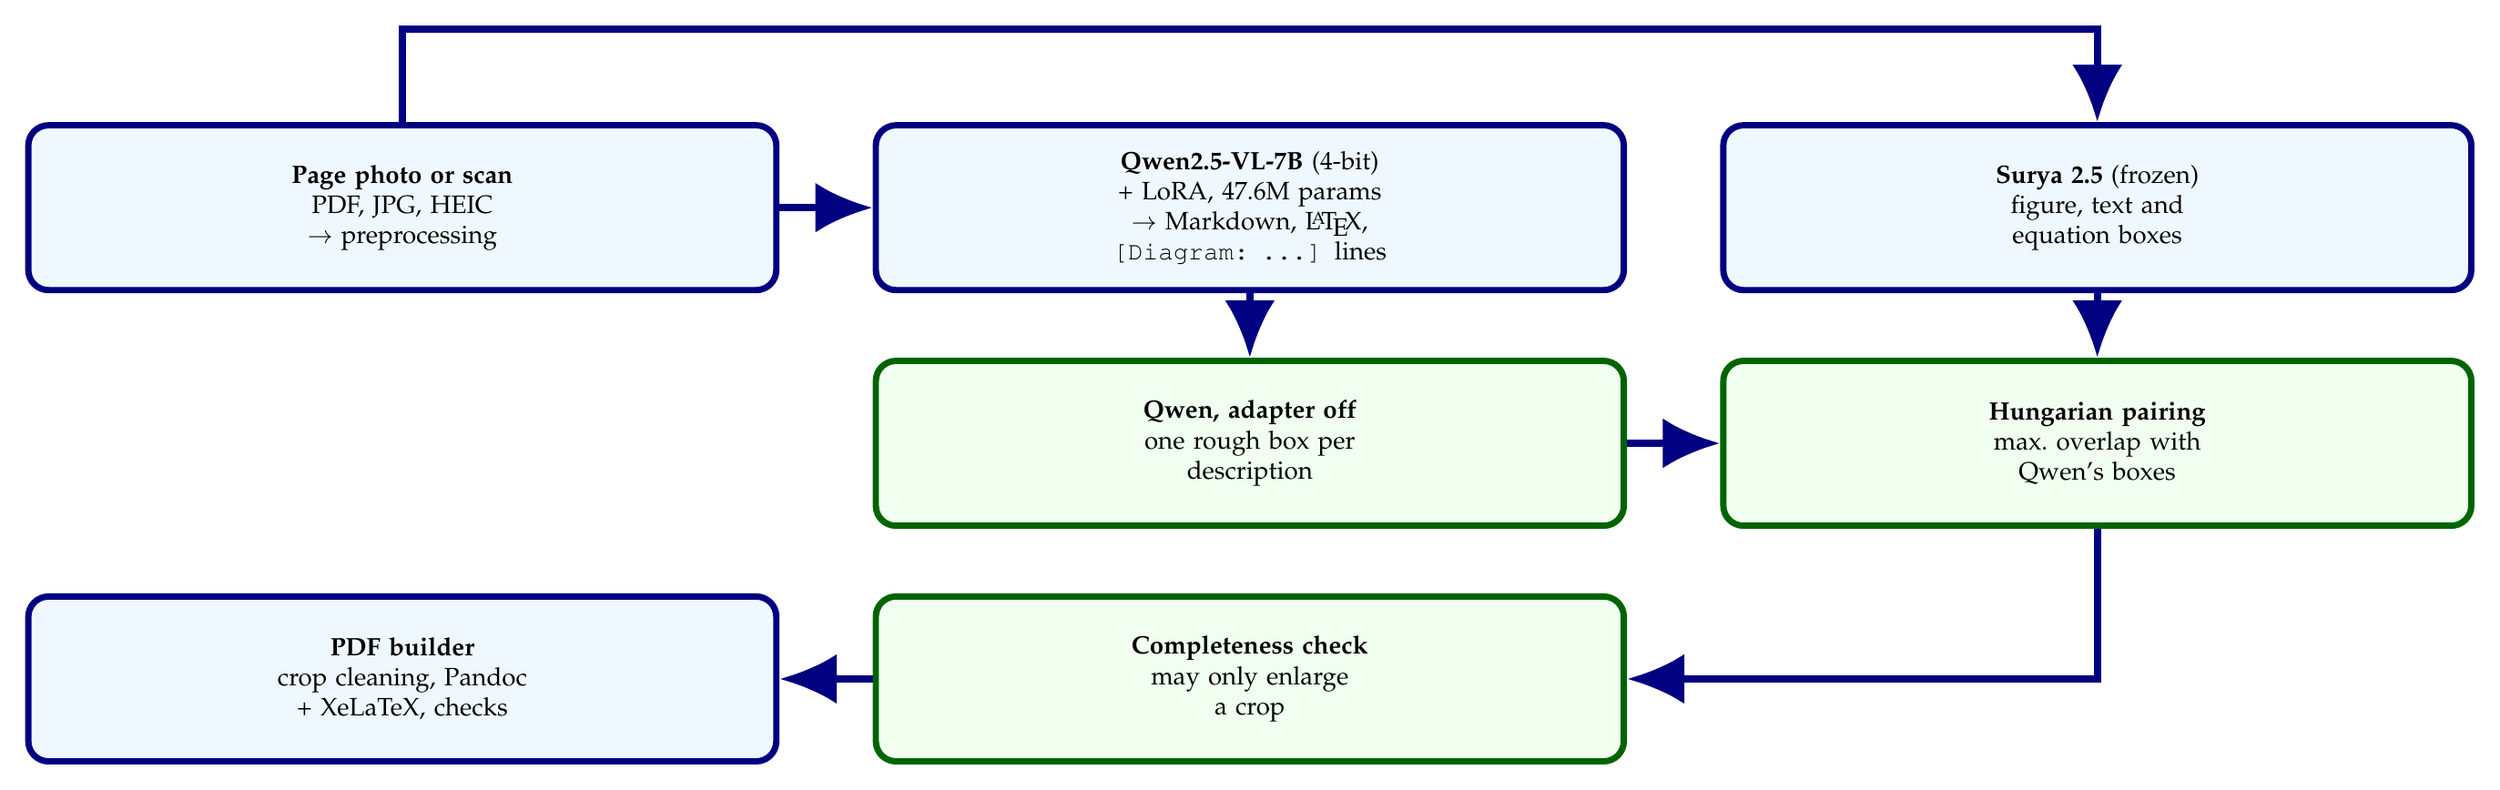
\begin{tikzpicture}[
  node distance=0.9cm and 1.3cm,
  box/.style={draw=NavyBlue, line width=2.5pt, rounded corners=8pt, fill=AliceBlue, align=center,
              minimum height=2.3cm, text width=10.2cm},
  nov/.style={box, fill=Honeydew, draw=DarkGreen},
  arr/.style={-{Latex[length=0.8cm,width=0.7cm]}, line width=3pt, NavyBlue}]
  \node[box] (img) {\textbf{Page photo or scan}\\PDF, JPG, HEIC\\$\to$ preprocessing};
  \node[box, right=of img] (q) {\textbf{Qwen2.5-VL-7B} (4-bit)\\+ LoRA, 47.6M params\\$\to$ Markdown, \LaTeX,\\\texttt{[Diagram: ...]} lines};
  \node[box, right=of q] (s) {\textbf{Surya 2.5} (frozen)\\figure, text and\\equation boxes};
  \node[nov, below=of q] (g) {\textbf{Qwen, adapter off}\\one rough box per\\description};
  \node[nov, below=of s] (h) {\textbf{Hungarian pairing}\\max.\ overlap with\\Qwen's boxes};
  \node[nov, below=of g] (v) {\textbf{Completeness check}\\may only enlarge\\a crop};
  \node[box, left=of v] (pdf) {\textbf{PDF builder}\\crop cleaning, Pandoc\\+ XeLaTeX, checks};
  \draw[arr] (img) -- (q); \draw[arr] (q) -- (g); \draw[arr] (s) -- (h); \draw[arr] (g) -- (h);
  \draw[arr] (h) |- (v); \draw[arr] (v) -- (pdf);
  \draw[arr] (img.north) -- ++(0,1.3) -| (s.north);
\end{tikzpicture}
\captionof{figure}{\color{Blue} Overall architecture. Green boxes are the novelty-phase additions.}
\label{Arch}
\end{center}
\begin{center}
\scalebox{0.82}{
\begin{tabular}{|l|l|c|l|}
\hline
\textbf{Stage} & \textbf{Model / tool} & \textbf{Trained by us?} & \textbf{What it contributes to the PDF} \\
\hline
Preprocessing & OpenCV rules & no & page found, deskewed, contrast and noise fixed \\
Recognition & Qwen2.5-VL-7B + QLoRA & \textbf{yes} & all text and \LaTeX, one \texttt{[Diagram: ...]} line per drawing \\
Layout & Surya 2.5 (frozen) & no & boxes of drawings: the pixels that are cropped \\
Grounding (novelty) & Qwen, adapter off & no & which box belongs to which \texttt{[Diagram]} line \\
Pairing (novelty) & Hungarian algorithm & no & one box per description, best total overlap \\
PDF & Pandoc + XeLaTeX & no & crops placed at their \texttt{[Diagram]} line, caption = description \\
\hline
\end{tabular}}
\captionof{table}{\color{Blue} Who does what. Only Qwen is trained. Everything after recognition copies its text verbatim.}
\end{center}
\begin{itemize}
	\item \textbf{QLoRA:} base weights frozen in 4-bit NF4, update $W x + \tfrac{\alpha}{r} B A x$ with
	$r=16$, $\alpha=32$ on all attention and MLP projections. Loss: next-token cross-entropy on the
	answer tokens only (image and prompt masked). Paged AdamW 8-bit, learning rate $10^{-4}$ (cosine),
	effective batch 8, 3 epochs (114 steps), best epoch by validation loss: 53 min on one 16 GB GPU.
	\item \textbf{Metrics:} NED = edit distance / length of the longer text (0 = perfect). Equation F1
	= exact match of display equations after normalisation. Figure Error Score (FES) = blind human grade
	per description (correct 0, loose or partial 0.5, wrong 1). Localisation error = $1 - \mathrm{IoU}$
	with the hand-drawn box.
\end{itemize}

%----------------------------------------------------------------------------------------
\section*{Dataset Details}
\begin{center}
\scalebox{0.95}{
\begin{tabular}{|l|c|c|c|c|}
\hline
\textbf{Source} & \textbf{Medium} & \textbf{Pages} & \textbf{Train / Val / Test} & \textbf{Drawings} \\
\hline
IE643 class scribes & stylus ink, dark board & 205 & 151 / 20 / 34 & 121 \\
MLT notes & stylus ink, white & 129 & 97 / 6 / 26 & 72 \\
IE802 notebook & phone photos & 56 & 40 / 4 / 12 & 71 \\
HumynLabs CS notes & notebook photos & 20 & 15 / 1 / 4 & 10 \\
\hline
\textbf{Total} & 3 media & \textbf{410} & \textbf{303 / 31 / 76} & \textbf{274} \\
\hline
\end{tabular}}
\captionof{table}{\color{Blue} Our dataset (no public set pairs handwritten lecture pages with structured labels). Labels were drafted offline with Gemini and Claude, never used at inference, and all 76 test labels were checked by hand. Split by lecture or notebook to avoid leakage.}
\end{center}
\newlength{\dsh}\setlength{\dsh}{0.335\linewidth}
\noindent\begin{minipage}[t]{0.615\linewidth}\centering
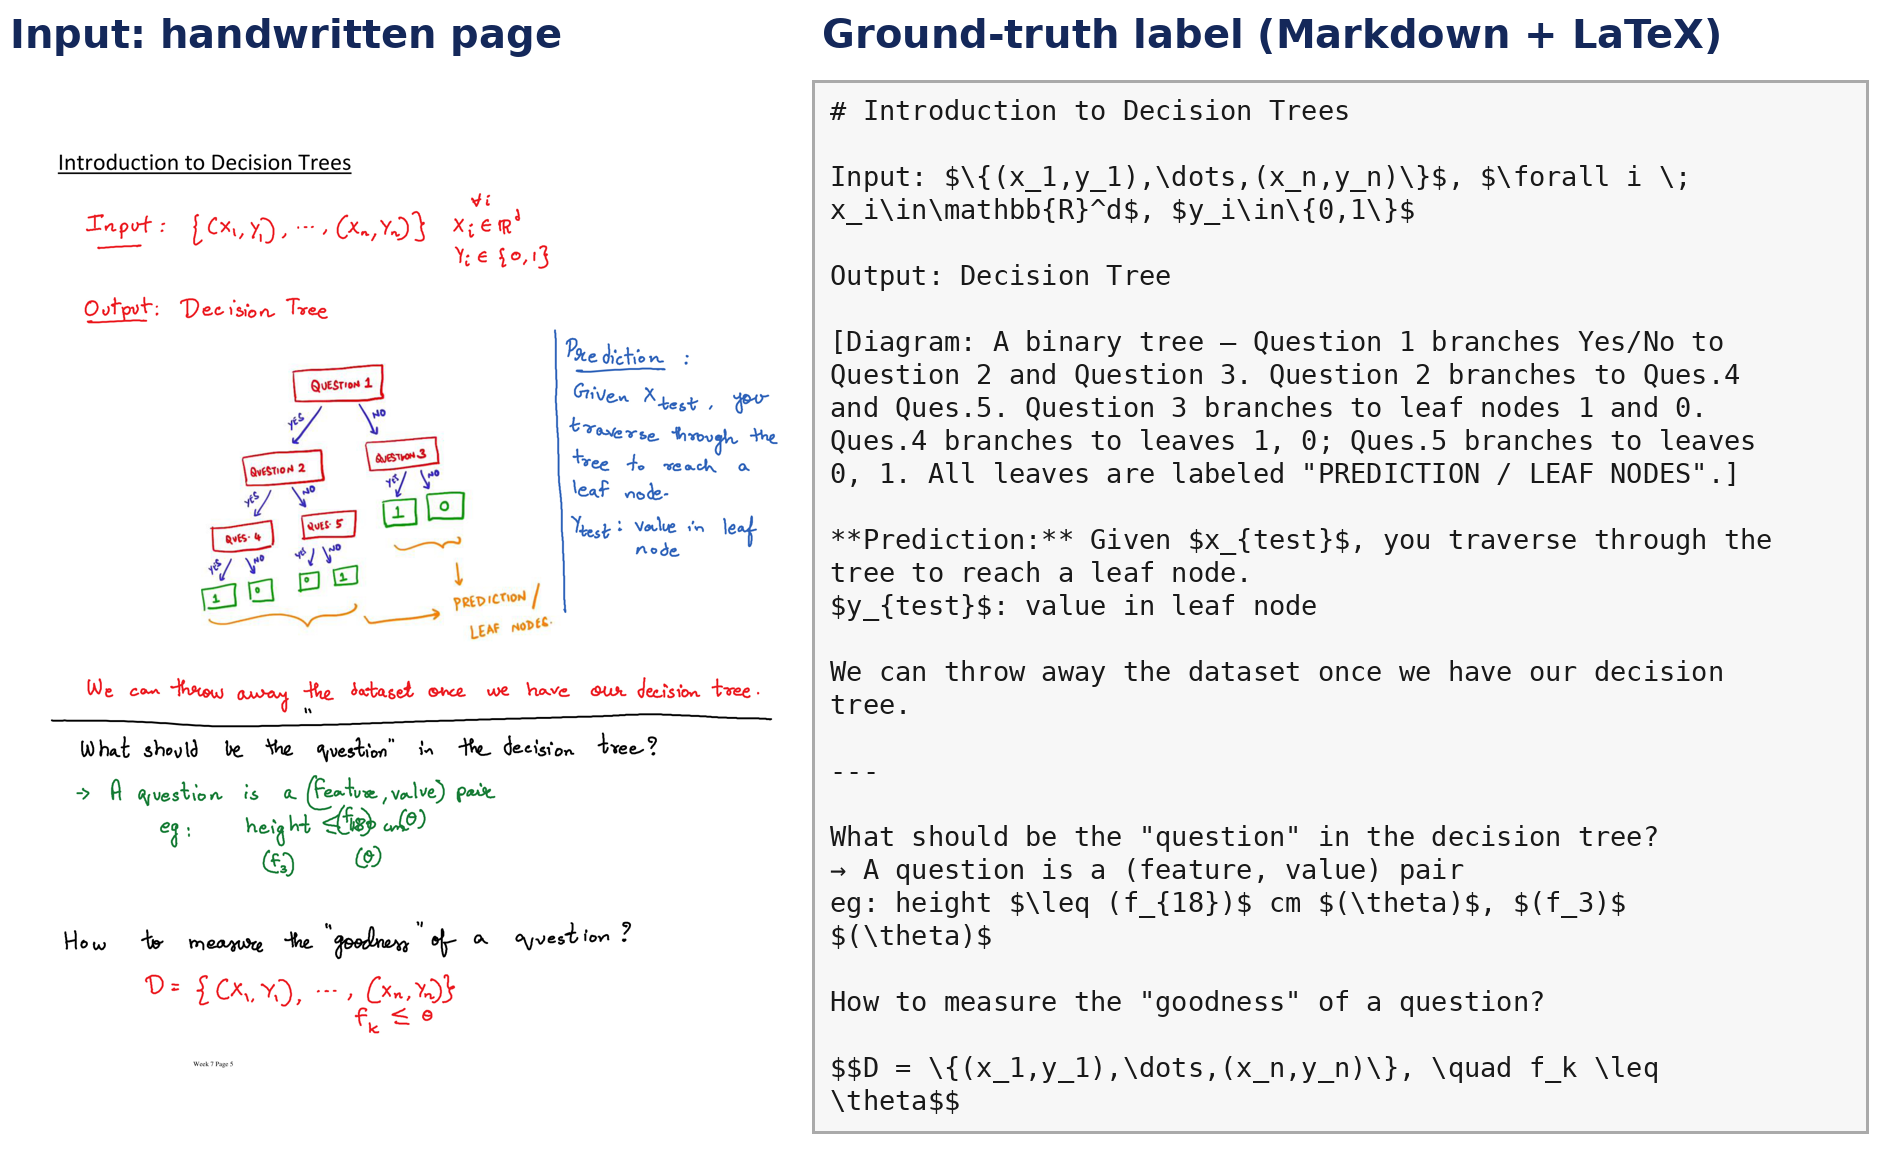
\includegraphics[height=\dsh]{dataset_example.png}
\captionof{figure}{\color{Blue} A training pair (MLT week 7, page 5). Text becomes Markdown, maths \LaTeX, and the drawing one \texttt{[Diagram]} line.}
\end{minipage}\hfill
\begin{minipage}[t]{0.36\linewidth}\centering
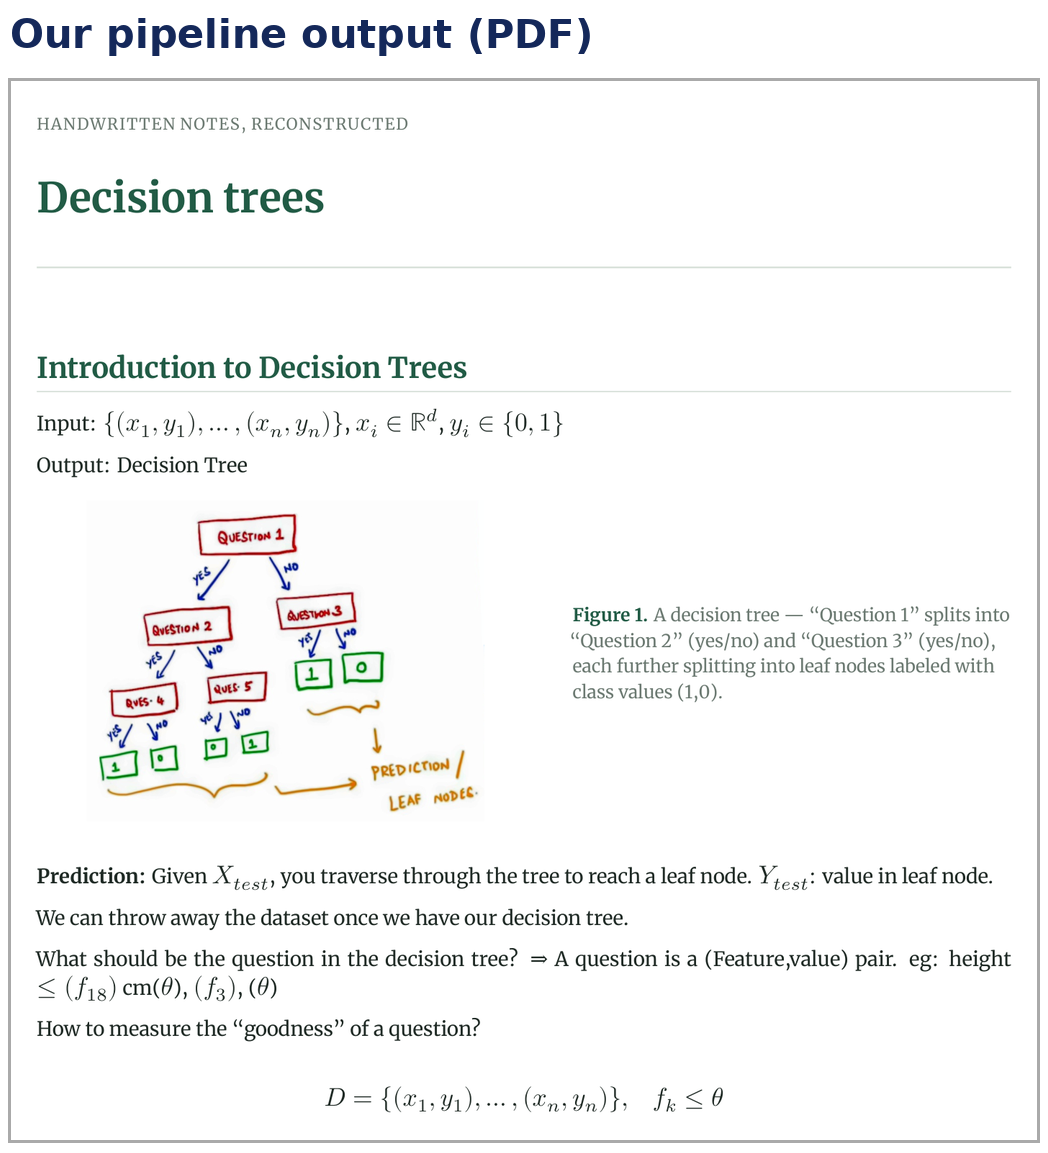
\includegraphics[height=\dsh]{mlt07p5_pipeline_panel.png}
\captionof{figure}{\color{Blue} The same page through our full pipeline (web demo, 58 s). The drawing is cropped and captioned automatically.}
\end{minipage}

\columnbreak
%----------------------------------------------------------------------------------------
\section*{Novelty Assessment}
The intensive assessment feedback asked us to fix figures on dense notebook pages (IE802) and show where errors arise. We drew
ground-truth boxes on 24 IE802 val/test pages and 8 training pages (used only for tuning).
\begin{enumerate}[leftmargin=1.5em,itemsep=0.25em]
	\item \textbf{Diagnosis.} For each figure we compared the page, Surya's boxes, the descriptions and
	the PDF, and named the step that failed. Pairing by reading order caused most errors: Surya reads
	some pages in a different order than Qwen, and a drawing split into two boxes shifts every later pair.
	\begin{center}
	\begin{tabular}{|c|c|c|c|c|}
	\hline
	correct & \textbf{matching} & localisation & recognition & placement \\
	\hline
	11 & \textbf{8} & 4 & 1 & 0 \\
	\hline
	\end{tabular}
	\captionof{table}{\color{Blue} Step that decided each of the 24 placed IE802 figures (old method).}
	\end{center}
	\item \textbf{Method B, ``Surya decides where, Qwen decides which''.} The same Qwen with its adapter
	switched off (the base model, pretrained for grounding) gives a rough box per \texttt{[Diagram]}
	description [1]. The Hungarian algorithm [4] pairs descriptions with Surya boxes [3] so that the total
	overlap with Qwen's boxes is largest, so reading order no longer matters. Surya pieces inside one Qwen
	box are joined, and if no Surya box overlaps enough ($\mathrm{IoU}<0.2$, tuned on training pages)
	Qwen's own box is used.
	\item \textbf{Better boxes.} Surya 2.5 replaces Surya 2 (box precision 0.73 $\to$ 0.83 on all 410 pages). When Qwen gives two
	descriptions the same box, the page is grounded again with one prompt that lists every description.
	\item \textbf{Completeness check.} The base Qwen scores ``is the whole sketch shown?'' for larger
	candidate crops that contain the chosen one. A crop is enlarged only if the score rises by 0.05, so a
	drawing can be completed but never cut. A first version that could also shrink crops was dropped
	after it lost a blind check.
	\item \textbf{Which figures to check.} Qwen's $P(\text{yes})$ for ``does this crop show the
	described sketch'' ranks failures well (AUC 0.82). 5 of its 8 flags are real errors against a 23\% base
	rate.
	\item \textbf{Source-attributed footnotes.} Each section of the test lectures retrieves one passage
	from \emph{Dive into Deep Learning} [5] with BM25 [6]. Qwen writes one or two sentences from that
	passage only, or NONE, and cites the section. 18 of 21 footnotes were relevant and supported.
\end{enumerate}

\begin{center}
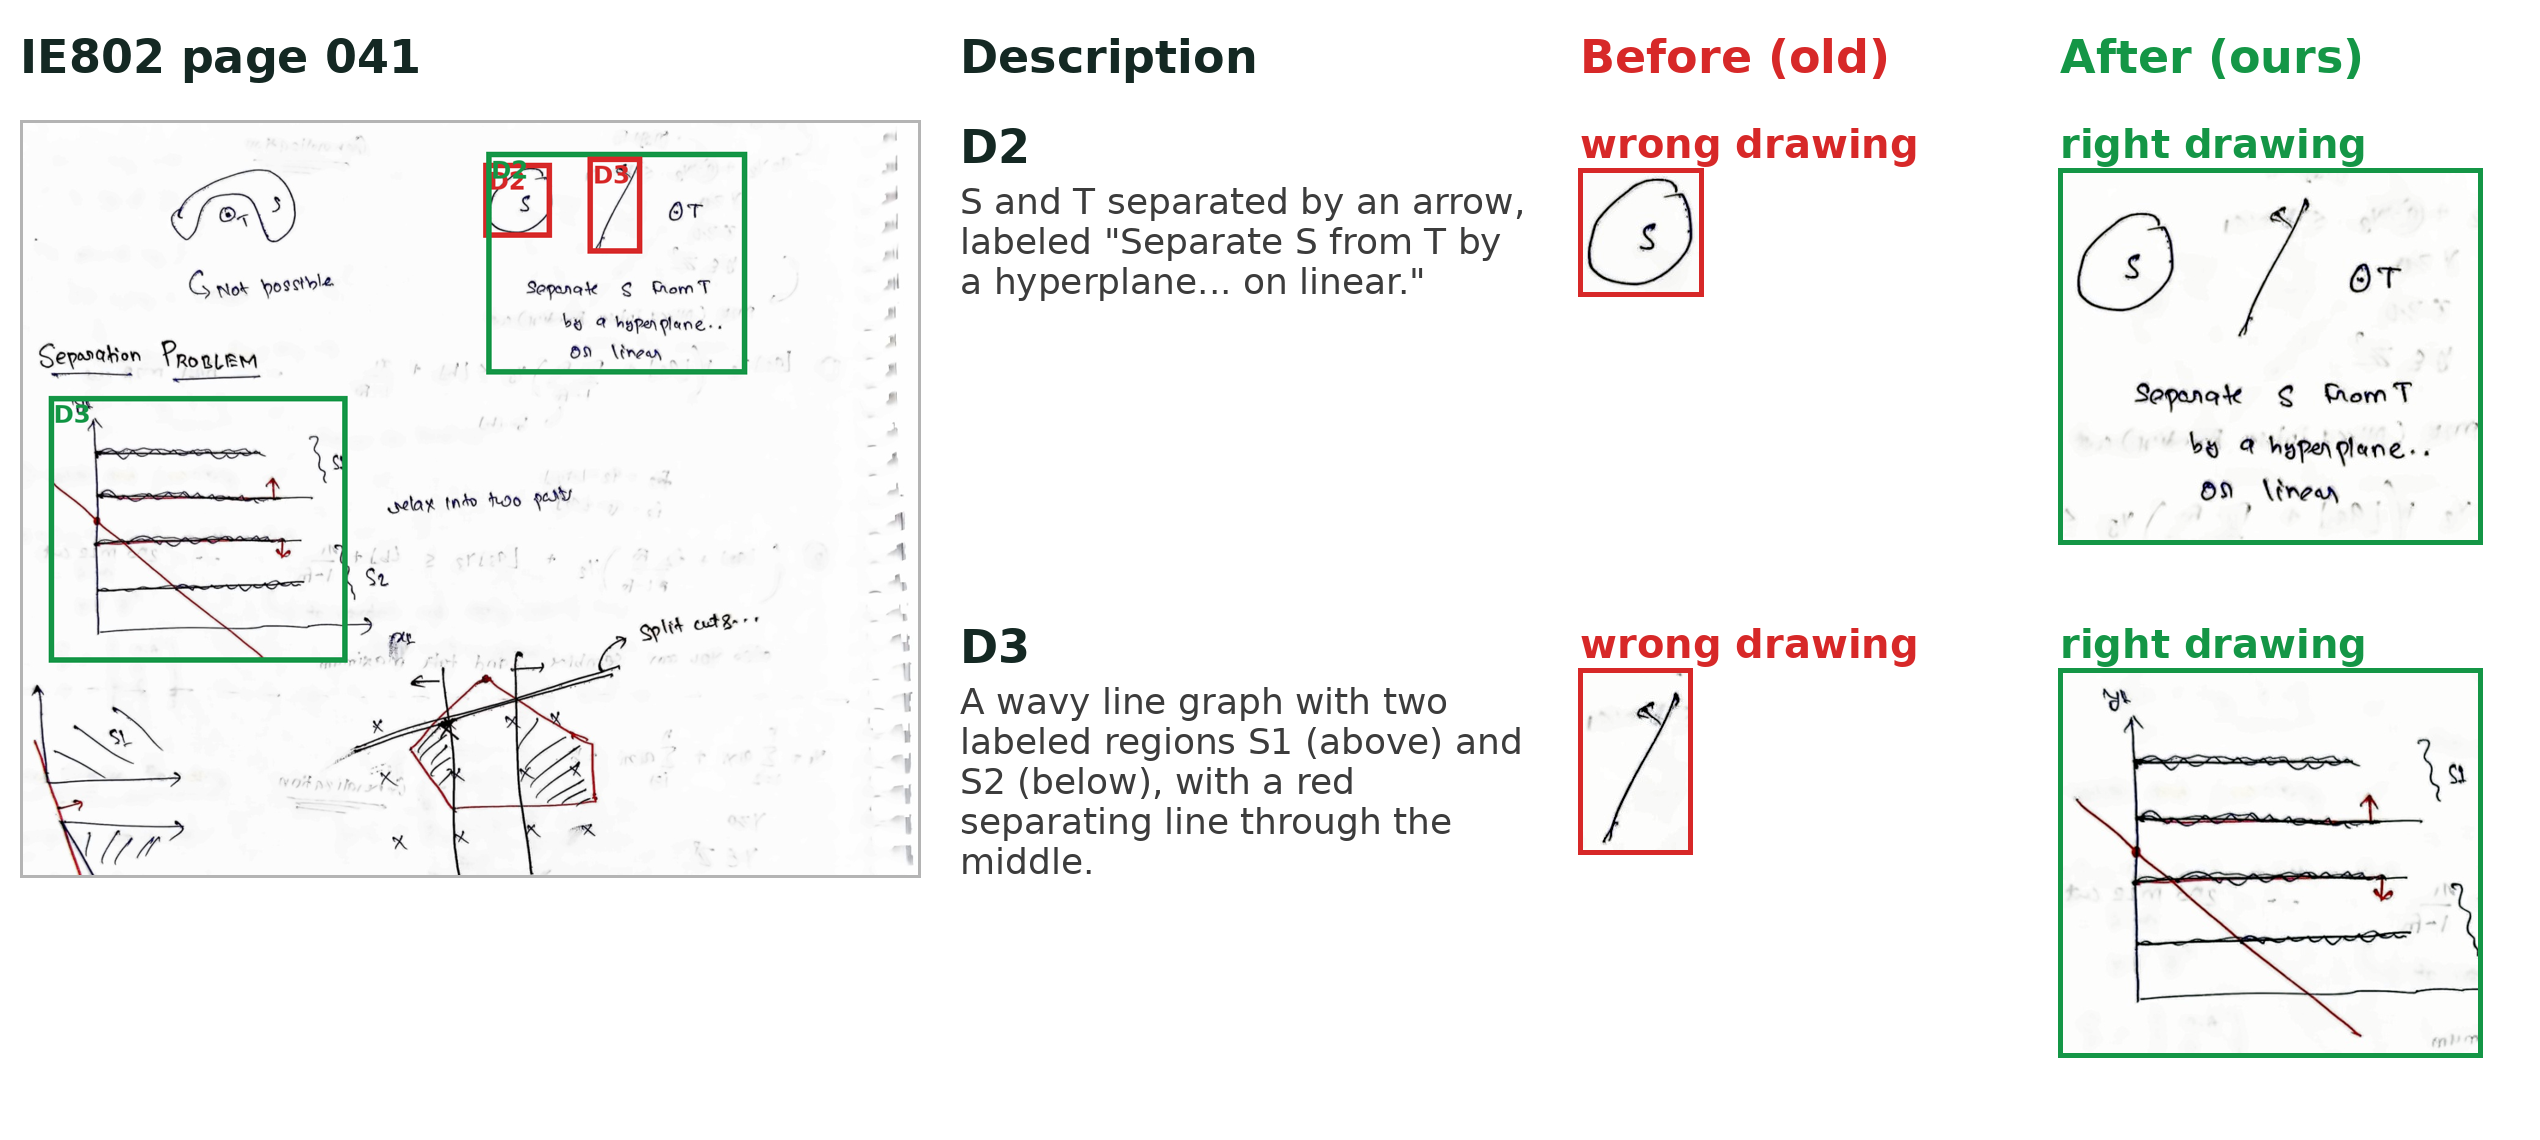
\includegraphics[width=0.6\linewidth]{page041_before_after.png}
\captionof{figure}{\color{Blue} IE802 page 041. Reading-order pairing put the wrong drawing under both captions (red). Our final pipeline places the right drawing with its labels (green).}
\label{arch}
\end{center}

%----------------------------------------------------------------------------------------
\section*{Results}
\begin{center}
\scalebox{0.9}{
\begin{tabular}{|l|c|c|c|c|c|c|c|}
\hline
\textbf{Model} & \textbf{NED}$\downarrow$ & \textbf{CER}$\downarrow$ & \makecell{\textbf{Text}\\\textbf{CER}$\downarrow$} & \makecell{\textbf{Token}\\\textbf{F1}} & \textbf{BLEU-4} & \makecell{\textbf{Eq.}\\\textbf{F1}} & \makecell{\textbf{Eq.}\\\textbf{edit}} \\
\hline
Qwen2.5-VL-7B zero-shot & 0.596 & 0.915 & 0.774 & 0.623 & 0.407 & 0.143 & 0.336 \\
+ Surya boxes as input & 0.313 & 0.347 & 0.253 & \textbf{0.858} & 0.690 & 0.324 & 0.686 \\
\textbf{Fine-tuned, image only (ours)} & \textbf{0.311} & \textbf{0.332} & \textbf{0.227} & 0.855 & \textbf{0.707} & \textbf{0.338} & \textbf{0.703} \\
\hline
\end{tabular}}
\captionof{table}{\color{Blue} Recognition, 76 test pages. Fine-tuning roughly halves the error (paired NED gain 0.284, 95\% CI 0.247--0.324, 74 of 76 pages better). Layout input does not help.}
\end{center}
\begin{center}
\scalebox{0.95}{
\begin{tabular}{|l|c|c|c|}
\hline
\textbf{Figure choice} & \textbf{Right drawing} & \textbf{Box IoU $\ge$ 0.5} & \textbf{Loc.\ error} $\downarrow$ \\
\hline
A: reading order (old) & 15 & 10 & 0.58 \\
B: Qwen grounding + Hungarian & 21 & 14 & 0.42 \\
B + Surya 2.5 & 21 & 16 & 0.39 \\
B + Surya 2.5 + shared-box fix$^{*}$ & \good{23} & 18 & 0.32 \\
\textbf{+ completeness verifier} & \good{23} & \textbf{19} & \textbf{0.30} \\
\hline
\end{tabular}}
\captionof{table}{\color{Blue} Figures, 23 IE802 val/test descriptions with a hand-drawn box. Settings chosen on 8 training pages. $^{*}$Refined after inspecting one val/test case.}
\end{center}
\begin{center}
\scalebox{0.9}{
\begin{tabular}{|l|c|c|c|c|}
\hline
\textbf{Blind human grades, 24 IE802 descriptions} & \textbf{Correct} & \textbf{Loose/partial} & \textbf{Wrong} & \textbf{FES}$\downarrow$ \\
\hline
A: reading order (old) & 13 & 2 & 9 & 0.42 \\
\textbf{B: Qwen grounding + Hungarian} & \textbf{20} & 0 & \textbf{4} & \textbf{0.17} \\
\hline
\end{tabular}}
\captionof{table}{\color{Blue} Graded blind. Later blind side-by-side checks: Surya 2.5 beat Surya 2 by 10 to 2 ($p=0.039$), the completeness check won 3, lost 0.}
\end{center}

%----------------------------------------------------------------------------------------
\section*{Conclusion and Future Work}
\begin{itemize}
	\item A fine-tuned 7B vision-language model reads our handwriting well (NED 0.311). The main figure
	problem was pairing descriptions with drawings, not finding drawings.
	\item ``Surya decides where, Qwen decides which'' fixes it: 23 of 23 right drawings on the checked
	notebook pages, every step checked blind. About 90\% of maths symbols are read right, and a retrain
	with one maths notation raised exact equation match (0.17 $\to$ 0.23) but not overall NED.
	\item Future work: consistent equation grouping in labels, a detector trained on our boxes, TikZ
	redrawing of simple diagrams, and a user study of the footnotes.
\end{itemize}

%----------------------------------------------------------------------------------------
\section*{References}
{\footnotesize
\begin{enumerate}[label={[\arabic*]},leftmargin=2.2em,itemsep=0.1em]
\item Shuai Bai, Keqin Chen, Xuejing Liu, Jialin Wang, Wenbin Ge, Sibo Song, Kai Dang, Peng Wang,
Shijie Wang, Jun Tang, Humen Zhong, Yuanzhi Zhu, Mingkun Yang, Zhaohai Li, Jianqiang Wan, Pengfei
Wang, Wei Ding, Zheren Fu, Yiheng Xu, Jiabo Ye, Xi Zhang, Tianbao Xie, Zesen Cheng, Hang Zhang,
Zhibo Yang, Haiyang Xu and Junyang Lin. Qwen2.5-VL Technical Report, arXiv, 2025.
\url{https://arxiv.org/abs/2502.13923}
\item Tim Dettmers, Artidoro Pagnoni, Ari Holtzman and Luke Zettlemoyer. QLoRA: Efficient
Finetuning of Quantized LLMs, NeurIPS, 2023. \url{https://arxiv.org/abs/2305.14314}
\item Vik Paruchuri and Datalab. \url{https://github.com/datalab-to/surya}, Accessed on: 3rd October, 2026.
\item Harold W. Kuhn. The Hungarian method for the assignment problem, Naval Research Logistics
Quarterly, 1955. \url{https://doi.org/10.1002/nav.3800020109}
\item Aston Zhang, Zachary C. Lipton, Mu Li and Alexander J. Smola. Dive into Deep Learning,
Cambridge University Press, 2023. \url{https://d2l.ai}
\item Stephen Robertson and Hugo Zaragoza. The Probabilistic Relevance Framework: BM25 and Beyond,
Foundations and Trends in Information Retrieval, 2009. \url{https://doi.org/10.1561/1500000019}
\end{enumerate}}

%----------------------------------------------------------------------------------------
\section*{Acknowledgments}
\small \textnormal{We thank Professor P. Balamurugan for his guidance throughout the course and the project, and the
teaching assistants for their feedback after the intensive assessment, which shaped the novelty work.}

\section*{Github Link and Demo Video Link}
\vspace{-0.5cm}
\begin{center}
		\begin{minipage}{0.4\linewidth}
			\centering
			\textbf{Github Repository}\\[1ex]
			\qrcode[height=3.6cm]{\repourl}
		\end{minipage}\hfill
		\begin{minipage}{0.4\linewidth}
			\centering
			\textbf{Demo Video Link}\\[1ex]
			\qrcode[height=3.6cm]{\demourl}
		\end{minipage}
\end{center}

\end{multicols}
\vspace{0.1cm}
\end{framed}
\end{minipage}
\end{document}
